\begin{frame}{Simple Probability Tree}
\begin{center}
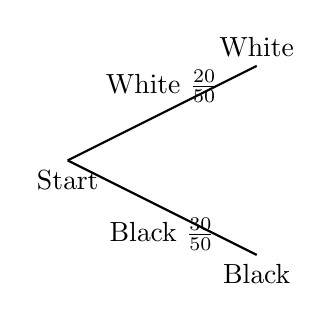
\begin{tikzpicture}[scale=1.2]
    \coordinate (A) at (0,0);
    \coordinate (B) at (2,1);
    \coordinate (C) at (2,-1);
    
    \draw[thick] (A) -- node[above] {White $\frac{20}{50}$} (B);
    \draw[thick] (A) -- node[below] {Black $\frac{30}{50}$} (C);
    
    \node[below] at (A) {Start};
    \node[above] at (B) {White};
    \node[below] at (C) {Black};
\end{tikzpicture}
\end{center}

\footnotesize
\texttt{\textbackslash draw[thick] (A) -- node[above] \{White \$\textbackslash frac\{20\}\{50\}\$\} (B);}
\end{frame}